\section{Distributed Algorithm with Partial Information}
\label{sec:algorithm}
In this section, we shall introduce a novel approximation method to decouple the centralized optimization on the RHS of the Bellman's equations in equation (\ref{eqn:sp_0}) to each AP for arbitrary system state.
For the APs outside the conflict AP sets of each other, the update of dispatching actions at one AP will not affect the task computation originated from other APs.
On the other hand, for the APs within the same conflict AP set, the optimization of their dispatching actions is coupled.
% Due to the unknown signaling latency, it is difficult for one AP (say the $k$-th AP) to predict the update of the dispatching actions at the other APs ($\forall k' \in\ccSet_{k}$).
% Hence, cooperative optimization of dispatching actions for the APs within the same conflict AP set is infeasible.
Hence, we introduce an alternative actions update algorithm to optimize the dispatching actions of subset of $\apSet$ in each broadcast interval periodically, while other APs maintain their dispatching actions in the previous broadcast interval.
Specifically, the proposed distributed algorithm consists of the following two steps:
%\hongyc{(move two steps adjacent in the following subsections)}
\begin{enumerate}
    \item We first introduce a time-variant baseline policy, use its value function to approximate the value function of the optimal policy $\Policy^*$ in each broadcast interval, and derive the analytical expression of the approximate value function for arbitrary GSI in Section \ref{subsec:baseline}.
    \item With the approximate value function, an alternative actions update algorithm, where only a subset of APs are selected to update their dispatching actions distributedly in each broadcast interval, is proposed in Section \ref{subsec:ap_alg}.
    Moreover, the analytical performance bound is derived in Section \ref{subsec:analysis}.
\end{enumerate}
% In our proposed approximate solution framework, we extend this procedure to the POMDP problem in P1 by exploiting the structure of partially observed edge computing networks.
% To the best knowledge of authors, a POMDP can hardly be solved via the Bellman's equations of full system state knowledge in the existing literature.

\subsection{Baseline Policy and Approximate Value Function}
\label{subsec:baseline}
To alleviate the curse of dimensionality, we first use the baseline policy with fixed dispatching actions to approximate the value function at the RHS of the Bellman's equations in equation (\ref{eqn:val_f}).
The baseline policy is elaborated below.

\begin{policy}[Baseline Policy]
    In the baseline policy $\Baseline$, each AP fixes their dispatching actions as in the previous broadcast interval. Specifically, at the $t$-th broadcast interval,
    {\small
    \begin{align}
        \Baseline\Paren{\Stat(t),\Delay(t)} &\define \Brace{ 
            \Pi_{1}(\Stat_{1}(t),\mathcal{D}_{1}(t)),
            \dots,
            \Pi_{K}(\Stat_{K}(t),\mathcal{D}_{K}(t))
        },
    \end{align}
    }%
    where
    {\small
    \begin{align}
        \Pi_{k}\Paren{\Stat_{k}(t),\mathcal{D}_{k}(t)}
        &\define \Brace{
            {\omega}_{k,j}(t+1) \Big| \forall j\in\jSpace
        }, \forall k\in\apSet.
    \end{align}
    }%
\end{policy}

Let $W_{\Baseline}(\cdot)$ be the value function of the baseline policy $\Baseline$, we shall approximate the value function of the optimal policy $V(\cdot)$ via $W_{\Baseline}$, i.e.,
{\small
\begin{align}
    &V\Paren{\Stat(t+1)} \approx W_{\Baseline}\Paren{\Stat(t+1)}
    \nonumber\\
    =& \sum_{m\in\esSet,j\in\jSpace}\Brace{
        \sum_{k\in\apSet} \tilde{W}^{\AP}_{k,m,j}(\Stat(t+1))
        +\tilde{W}^{\ES}_{m,j}(\Stat(t+1))
    },
    \label{eqn:baseline}
\end{align}
}%
where $\tilde{W}^{\AP}_{k,m,j}(\Stat(t+1))$ denotes the cost raised by the type-$j$ jobs which are being transmitted from the $k$-th AP to the $m$-th processing server with the baseline policy $\Baseline$ and initial system state $\Stat(t+1)$, and $\tilde{W}^{\ES}_{m,j}(\Stat(t+1))$ denotes the cost raised by the type-$j$ jobs on the $m$-th server.
Their definitions are given below.
{\small
\begin{align}
    \tilde{W}^{\AP}_{k,m,j} \Paren{\Stat(t+1)} &\define
        \sum_{i=0}^{\infty} \gamma^{i+1} \mathbb{E}^{\Baseline}\Bracket{
            \Inorm{\vec{R}^{(k)}_{m,j}(t+i+1)}
        },
    \label{w_ap}
    \\    
    \tilde{W}^{\ES}_{m,j} \Paren{\Stat(t+1)} &\define
        \sum_{i=0}^{\infty} \gamma^{i+1} \mathbb{E}^{\Baseline}\Bracket{
            Q_{m,j}(t+i+1) +
            \nonumber\\
            &~~~~~~~~~~\beta I[Q_{m,j}(t+i+1) = L_{max}]
        }.
    \label{w_es}
\end{align}
}%
% Moreover, the explicit expressions of $\tilde{W}^{\AP}_{k,m,j}(\Stat(t+1))$ and $\tilde{W}^{\ES}_{m,j}(\Stat(t+1))$ are derived in the following lemmas, respectively.

\subsection{Distributed Actions Update}
\label{subsec:ap_alg}
Although the optimal value function has been approximated via the baseline policy in the previous part, it is still infeasible to solve the RHS of the Bellman's equations as the evaluation of equation (\ref{w_ap}) and (\ref{w_es}) requires the knowledge of GSI and \brlatency~at all APs.
% for all the APs to solve the RHS of the Bellman's equations in a distributed manner with OSI and local \brlatency~only.
% This is because the evaluation of equation (\ref{w_ap}) and (\ref{w_es}) requires the knowledge of GSI and \brlatency~at all APs.
Instead, it is feasible for part of APs to update their dispatching actions distributedly in each broadcast interval and achieve a better performance compared with baseline policy.
Hence, we first define the following sequence of AP subsets, where each subset are selected to update dispatching actions periodically.
\begin{definition}[Subset Partition]
    Let $\mathcal{Y}_{1}, \dots, \mathcal{Y}_{N} \subseteq \apSet$ be a collection of subsets of AP set $\apSet$, which satisfy
    {\small
    \begin{align}
        &\bigcup_{n=0,\dots,N-1} \mathcal{Y}_{n} = \apSet
        \label{eqn:subset_cup}
        \\
        \esSet_{y} \cap \esSet_{y'} &=\emptyset, y' \neq y~(\forall y',y \in \mathcal{Y}_{n}).
        \label{eqn:subset_disjoint}
    \end{align}
    }%
\end{definition}
% The condition in equation (\ref{eqn:subset_cup}) is to ensure all the APs can update their dispatching actions periodically, whereas the condition in equation (\ref{eqn:subset_disjoint}) is to ensure APs in the conflict AP sets of each other will not update their dispatching actions in the same broadcast interval.
% For example, as illustrated in Fig.\ref{fig:system}, the AP set $\apSet$ could be decomposed of two subsets as $\set{1,3}$ and $\set{2}$.
The subset partition is not trivial and a partition to minimize the update period $N$ is preferred.
A heuristic greedy algorithm is given in Algorithm \ref{alg_0}.
\begin{algorithm}[ht]
    \caption{Greedy Subset Partition Algorithm}\label{alg_0}
    \DontPrintSemicolon % Some LaTeX compilers require you to use \dontprintsemicolon instead
    \KwIn{$\apSet, \set{\esSet_{k}, \forall k\in\apSet}$ }
    \KwOut{a subset partition $\set{ \mathcal{Y}_{n} }$}
    Initialize a subset partition as $\mathcal{Y}_{n} = \set{n}$ ($\forall n\in\apSet$).\;
    \While{ $\exists \mathcal{Y}_a$ and $\mathcal{Y}_b$ ($a \neq b$) that $\cup\set{ \esSet_{y}|y\in\mathcal{Y}_a } \bigcap \cup\set{ \esSet_{y}|y\in\mathcal{Y}_b } \neq \emptyset$ }
    {
        Count number of subsets in the current subset partition which have disjoint candidate set with $\mathcal{Y}_n$ ($\forall n$), denoted the number as $I_{n}$.\;
        $\tilde{n} \gets \arg\min_{n} I_{n}$\;
        Merge the subset $Y_{\tilde{n}}$ with one of its disjoint subsets.\;
    }
\end{algorithm}

At the $t$-th broadcast interval, the APs in the subset indexed with $n \define t \pmod{N}$ update their dispatching actions, while the other APs keep the same dispatching actions as the previous broadcast interval.
Hence, let
{\small
\begin{align}
    \tilde{\mathcal{A}}(t) \define \Brace{ {\omega}_{y,j}(t+1) \Big| \forall y\in\mathcal{Y}_{n},j\in\jSpace }
\end{align}
}%
be the aggregation of dispatching actions of the APs in the subset $\mathcal{Y}_{n}$, and
{\small
\begin{align}
    \hat{\mathcal{A}}(t) \define \Brace{ {\omega}_{y,j}(t+1) \Big| \forall y\notin\mathcal{Y}_{n}, j\in\jSpace}
\end{align}
}%
be the aggregation of dispatching actions of the rest APs, which are same as in the previous broadcast interval.
At the $t$-th broadcast interval, the optimization of dispatching actions $\tilde{\mathcal{A}}(t)$ at the RHS of the Bellman's equations can be rewritten as the following problem.
{\small
\begin{align}
    \textbf{P2:}~
    \min_{ \tilde{\mathcal{A}}(t) }
    &\sum_{\Stat(t+1)} \Pr\Brace{
        \Stat(t+1) \Big| \Stat(t), \hat{\mathcal{A}}(t), \tilde{\mathcal{A}}(t)
    } \cdot W_{\Baseline}\Paren{\Stat(t+1)}.
\end{align}
}%

Moreover, we have the following conclusion on the decomposition of P2.
\begin{lemma}[]
    The optimization problem in P2 can be equivalently decoupled into local optimization problems at APs {for each subset partition}.
    Specifically, {the local optimization for each AP (say the $y$-th AP) in the $n$-th subset ($\forall n$) can be written as}
    {\small
    \begin{align}
        &\textbf{P3:}~
        \min_{ {\mathcal{A}}_{y}(t+1) }
        \mathbb{E}_{\set{ \Stat_{y}(t+1)|\Stat_{y}(t), \hat{\mathcal{A}}(t), {\mathcal{A}}_{y}(t+1) }}
        \nonumber\\
        &~~~~\sum_{ j\in\jSpace,m\in\esSet_{y} } \Brace{
            \tilde{W}^{\AP}_{k,j}\Paren{\Stat_{y}(t+1)}
            +\tilde{W}^{\ES}_{m,j}\Paren{\Stat_{y}(t+1)}
        }.
        \label{eqn:partial}
    \end{align}
    }%
    \label{lemma:w_partial}
\end{lemma}
\begin{proof}
    At the $t$-th broadcast interval, the $y$-th AP in the subset $\mathcal{Y}_{n}$ updates its dispatching actions, which could only affect the future cost raised on itself and its corresponding \emph{candidate server set}, i.e., the part of its OSI.
    Hence, it's obvious that the equation (\ref{w_ap}) and equation (\ref{w_es}) on the RHS of the Bellman's equations could be reduced into the form based only on the OSI of the $y$-th AP ($\forall y\in\mathcal{Y}_{n}$).
\end{proof}

The optimization of {dispatching actions $\mathcal{A}_{y}(t+1)$} for the $y$-th AP ($\forall y\in\mathcal{Y}_{n}$) in P3 could be achieved via searching all the processing servers in $\esSet_{y}$, {whose computational complexity is $O(J|\mathcal{M}_{y}|)$}.
As a result, the overall algorithm of job dispatching is elaborated in Algorithm \ref{alg_1}.
\begin{algorithm}[ht]
    \caption{Online Alternative Actions Update Algorithm}\label{alg_1}
    \DontPrintSemicolon % Some LaTeX compilers require you to use \dontprintsemicolon instead
    % \KwIn{$\Stat(t), \Delay(t)$}
    % \KwOut{$\tilde{\mathcal{A}}(t)$}
    Initialize all the APs with heuristic dispatching actions $\set{{\omega}_{k,j}(0)|\forall k\in\apSet,j\in\jSpace}$.\;
    \For{$t=0,1,2,\dots$}{
        % \tcc{Get the index of the subset to update at $t$.}
        $n \gets t \pmod{N}$\;
        % \tcc{Parallelly update the actions of APs in the subset $\mathcal{Y}_{n}$.}
        \ForPar{$y \in \mathcal{Y}_{n}$}{
            % \tcc{Each AP observes its LSI asynchronously.}
            The $y$-th AP observes $\Stat_{y}(t)$ after $\mathcal{D}_{y}(t)$.\;
            % \tcc{Then update actions by solving P3.}
            Solve P3 with $\Stat_{y}(t), \mathcal{D}_{y}(t)$ and obtain optimized actions $\set{\tilde{\omega}_{y,j}(t+1)|\forall j\in\jSpace}$\;
        }
        $\tilde{\mathcal{A}}(t+1) \gets \set{\tilde{\omega}_{y,j}(t+1)|\forall y\in\mathcal{Y}_{n},j\in\jSpace}.$\;
        % \tcc{The other APs fix the actions as the previous interval.}
        $\hat{\mathcal{A}}(t+1) \gets \hphantom{~~} \set{ {\omega}_{y,j}(t) | \forall y\in\mathcal{Y}_{n-1},j\in\jSpace }$\;
        $\hphantom{~~~~~~~~~~~~~~~~~} \cup \set{ {\omega}_{y,j}(t) | \forall y\notin\mathcal{Y}_{n-1},j\in\jSpace }$\;
    }
\end{algorithm}
% Moreover, we use the following example to illustrate the procedure of Algorithm \ref{alg_1}.
% \begin{example}
%     \label{exp:update}
%     Consider an edge computing system as Fig.\ref{fig:system}, where the AP set $\apSet$ could be partitioned into two subsets which are denoted as $\mathcal{Y}_{0} = \set{1,3}$ and $\mathcal{Y}_{1} = \set{2}$, respectively.
%     As illustrated in Fig.\ref{fig:update_timeline}, in the $1$-st interval the APs in subset $\mathcal{Y}_{0}$ would update their dispatching actions by solving P3, while the AP in subset $\mathcal{Y}_{1}$ fix its actions.
%     Denote the aggregation of their dispatching actions as $\tilde{\mathcal{A}}(1)$ and $\hat{\mathcal{A}}(1)$, respectively.
%     Then in the $2$-nd interval, the APs in subset $\mathcal{Y}_{0}$ fix their actions as $\tilde{\mathcal{A}}(1)$ which is denoted as $\hat{\mathcal{A}}(2)$, while 
%     the AP in subset $\mathcal{Y}_{1}$ updates the dispatching actions to $\tilde{\mathcal{A}}(2)$.
%     Hence, every AP update its dispatching actions with period $N=2$.
%     \begin{figure*}[htp!]
%         \centering
%         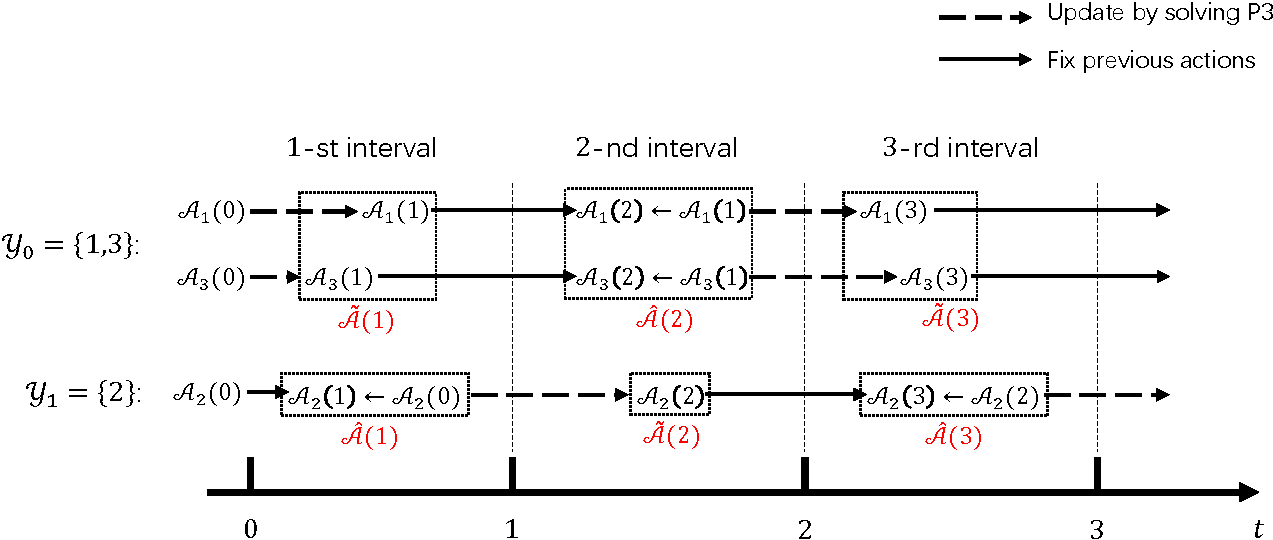
\includegraphics[width=0.60\textwidth]{update-timeline.pdf}
%         \caption{The Illustration of Example \ref{exp:update}.}
%         \label{fig:update_timeline}
%     \end{figure*}
% \end{example}

As a remark notice that since in Algorithm \ref{alg_1}, the computation complexity at each AP scales linearly with respect to {the size of candidate edge server set}, it can be deployed in a scenario with massive APs and edge servers, as long as the {the available number of edge servers for each AP} is limited.

\subsection{Analytical Performance Bound}
\label{subsec:analysis}
In most of the existing approximate MDP solutions \cite{mdp-bound1,mdp-bound2,mdp-bound3}, the performance is difficult to bound analytically as the approximate value function has no accurate meaning on the system cost or utility.
In the proposed algorithm, however, we derive the analytical expression for the baseline policy as the approximate.
Hence, the alternative dispatching actions update can ensure to achieve a better performance than the baseline policy.
This conclusion is summarized below.
% We have the following conclusion on the performance of the above proposed algorithm.
\begin{lemma}[Analytical Cost Upper Bound]
    \label{lemma:bound}
    Let $W_{\tilde{\Policy}}(\cdot)$ be the value function (average cost) of the proposed policy $\tilde{\Omega}$, i.e.,
    {\small
    \begin{align}
        W_{\tilde{\Policy}}(\Stat) \define
        \sum_{t'=1}^{\infty} \gamma^{t'-1} \mathbb{E}^{ \tilde{\Policy} } \Bracket{
            g\Paren{\Stat(t'), \tilde{\Policy}(\Stat(t'),t')} \Big| \Stat(1)=\Stat
        },  
    \end{align}
    }%
    we have
    {\small
    \begin{align}
        V(\Stat)
        \leq W_{\tilde{\Policy}}(\Stat)
        \leq W_{\Baseline}(\Stat),
        \forall \Stat.
    \end{align}
    }%
\end{lemma}
\begin{proof}
    $V(\Stat) \leq W_{\tilde{\Policy}}(\Stat)$ is straightforward as $\tilde{\Policy}$ is not optimal policy.
    The proof of $W_{\tilde{\Policy}}(\Stat) \leq W_{\Baseline}(\Stat)$ is equal to prove the improvement of one-step policy iteration, which is similar to the proof of \emph{Policy Improvement Property} in \cite{dp-control}.
\end{proof}
Therefore, $W_{\Baseline}(\Stat)$ derived in equation (\ref{eqn:baseline}) can be used as the analytical cost upper bound of the proposed policy $\Baseline$.
Moreover, Lemma \ref{lemma:bound} also implies that the proposed policy with fixed service edge server for each AP, as long as the {static dispatching policy} is used as the baseline policy.
% the average system cost of the proposed algorithm is upper bounded by $W_{\Baseline}(\Stat)$ ($\forall \Stat$) which means it is always better than the baseline policy. 

% \subsection{Scalability Analysis}
% \hongyc{(append the subsection to show that scalability is good, when connection is uniform with APs and edge servers.)}
%----------------------------------------------------------------------------------------%
%----------------------------------------------------------------------------------------%